\chapter{Einleitung}

\section{Aufgabe/Motivation}
Ziel des Versuchs ist die Bestimmung des Richtmoments $D$ eines Drehpendels sowie die Untersuchung des Trägheitsmoments $J$ eines unregelmäßig geformten Körpers für verschiedene Lagen der Drehachse. Dazu wird einerseits das Richtmoment über die Auslenkung des Pendels durch ein angreifendes Drehmoment bestimmt, andererseits über die Periodendauer einer Schwingung mit aufgesetzten Körpern bekannter Geometrie. Mit Hilfe des Steiner’schen Satzes lässt sich schließlich das Trägheitsmoment für verschiedene Achsen berechnen und mit den experimentell gewonnenen Werten vergleichen.

\section{Physikalische Grundlagen}
\cite{skript25}
\subsection*{Analogie zwischen Translations- und Rotationsbewegung}
Die Bewegungsgleichungen für Translationen und Rotationen sind formal analog, wenn die entsprechenden Größen ausgetauscht werden. Dabei gilt für das Torsionspendel:
\begin{equation}
    0 = J \cdot \ddot \varphi(t) + D \cdot \varphi(t)
\end{equation}
Diese homogene Differentialgleichung 2. Art hat die allgemeine Lösung
\begin{equation}
    \varphi(t) = \varphi_0 \cdot \cos(\omega t + \phi).
\end{equation}
Dabei ist $\omega = \sqrt{\frac{J}{D}}$ und $\phi$ die Startauslenkung.

\begin{table}[h!]
\renewcommand{\arraystretch}{1.75} % Zeilenhlöhe
\centering
\begin{tabular}{l|l}
    \textbf{Translation} & \textbf{Rotation} \\
    \hline
    Ort $x$ & Winkel $\varphi$ \\
    Ges. $v = \tfrac{dx}{dt}$ & Winkelges. $\omega = \tfrac{d\varphi}{dt}$ \\
    Bes. $a = \tfrac{d^2x}{dt^2}$ & Winkelbes. $\alpha = \tfrac{d^2\varphi}{dt^2}$ \\
    Masse $m$ & Trägheitsmoment $J$ \\
    Kraft $F$ & Drehmoment $M$ \\
    Impuls $p = mv$ & Drehimpuls $L = J\omega$ \\
    Trans.En. $E_{kin} = \tfrac{1}{2}mv^2$ & Rot.En. $E_{rot} = \tfrac{1}{2}J\omega^2$ \\
    $E_{ges} = \frac{1}{2}kx^2 + \frac{1}{2} mv^2$ & $E_{ges} = \frac{1}{2}D\phi^2 + \frac{1}{2} J \omega^2$ \\
    Schwingdauer $2\pi \sqrt{\frac{m}{k}}$ & Schwingdauer $2 \pi \sqrt{\frac{D}{J}}$
\end{tabular}
\caption{Vergleich der Größen in der Translation und Rotation}
\label{tab:translation-rotation}
\end{table}

\vspace{0.25cm}

Auch Federpendel und Drehpendel stehen in direkter Analogie:

\begin{equation}
    F = -kx \quad \Leftrightarrow \quad M = -D\varphi
    \label{eq:kraft_drehmoment_zusammenhang}
\end{equation}

\begin{equation}
T = 2\pi\sqrt{\frac{m}{k}} \quad \Leftrightarrow \quad T = 2\pi\sqrt{\frac{J}{D}}
\end{equation}

Das Richtmoment $D$ spielt dabei die Rolle der Federkonstante $k$.

\subsection*{Trägheitsmoment}
Das Trägheitsmoment $J$ eines Körpers bezüglich einer gegebenen Drehachse ergibt sich aus dem Volumenintegral:

\begin{equation}
    J = \int_V \rho(\vec{r}) r^2 \, dV,
\end{equation}

wobei $\rho(\vec{r})$ die Massendichte und $r$ der Abstand des Volumenelements zur Achse ist.  
Für einfache Körper ergeben sich bekannte Spezialfälle, etwa für eine homogene Scheibe mit Masse $m$ und Radius $r_s$:

\begin{equation}
    J_S = \tfrac{1}{2} m r_s^2
\end{equation}

Hierbei ist $J_S$ das Trägheitsmoment der Scheibe, $m$ ihre Masse und $r_s$ ihr Radius.

\subsection*{Steiner’scher Satz}
Für eine Achse, die parallel zur Symmetrieachse im Abstand $d$ verläuft, gilt:

\begin{figure}[h!]
    \centering
    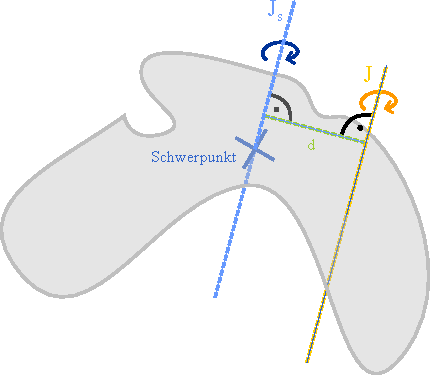
\includegraphics[width=0.4\textwidth, page=1,]{img/\versuchsnummer/steinsatz.pdf}
    \caption{Visualisierung des Stein'schen Satzes}
    \label{fig:steinscher_satz}
\end{figure}

\begin{equation}
    J = J_S + md^2
    \label{eq:steinsatz}
\end{equation}

mit $J_S$ als Trägheitsmoment bezüglich der Symmetrieachse, $m$ als Masse des Körpers und $d$ als Abstand der Achsen.
\subsection*{Bestimmung des Richtmoments}
Das Richtmoment $D$ des Drehpendels kann auf zwei Weisen bestimmt werden:

1. Über das Kraftgesetz:
\begin{equation}
    M = r \cdot F = -D\varphi,
\end{equation}
wobei $M$ das Drehmoment, $r$ der Radius der Aluminiumscheibe, $F = mg$ die Gewichtskraft eines tangential angreifenden Massestücks und $\varphi$ der Auslenkwinkel ist.

2. Über die Schwingungsdauer $T$ mit bekannter Massescheibe:

\begin{equation}
    D = \frac{4\pi^2 J_S}{T_2^2 - T_1^2} = \frac{2\pi^2 m r_s^2}{T_2^2 - T_1^2},
    \label{eq:richtmoment_rechnen}
\end{equation}
wobei $T_1$ die Periodendauer des Tisches allein, $T_2$ die Periodendauer mit aufgesetzter Scheibe, $J_S$ das Trägheitsmoment der Scheibe, $m$ ihre Masse und $r_s$ ihr Radius ist. 
Mathematisch werden die zwei einzelnen Periodendauern also via:
\begin{align}
    T_1 &= 2\pi \sqrt{\frac{J_T}{D}}, \\
    T_2 &= 2\pi \sqrt{\frac{J_T+J_S}{D}}
    \label{eq:T_def}
\end{align}

bestimmt. Wir können nun die Gleichung für \hyperref[eq:T_def]{$T_1$ (Gleichung 10)} und \hyperref[eq:T_def]{$T_2$ (Gleichung 11)} quadrieren und jeweils nach $J_T$ umstellen:
\begin{align}
    T_1^2 &= 4\pi^2 \frac{J_T}{D} &&\Rightarrow J_T = \frac{T_1^2 \cdot D}{4\pi^2} \\
    T_2^2 &= 4\pi^2 \frac{J_T+J_S}{D} &&\Rightarrow J_T = \frac{T_1^2 \cdot D}{4\pi^2} - J_S.
    \label{eq:traegheitsmoment_tisch}
\end{align}

Logischer weise können wir die Gleichung gleichsetzen und kommen damit auf 
\begin{equation}
    \frac{T_1^2 \cdot D}{4\pi^2} = \frac{T_1^2 \cdot D}{4\pi^2} - J_S.
\end{equation}

Formt man diese Gleichung nach $D$ um, so kommt man wieder zu \hyperref[eq:richtmoment_rechnen]{Gleichung 9}


\section{Versuchsanordnung}
Der Versuch wird mit einem Drehpendel mit senkrechter Achse durchgeführt. Zum Aufbau gehören eine Drehgabel mit Drehtisch, eine Aluminiumscheibe mit Winkelteilung und Schnurnut, eine runde sowie eine unregelmäßig geformte Messingscheibe, ein Gewichtsteller mit Zugschnur, sechs Auflegegewichte zu je 50g, eine Waage, eine Handstoppuhr, ein Messschieber sowie eine Balancierschneide. Mit diesem Aufbau lassen sich die notwendigen Messungen zur Bestimmung des Richtmoments und der Trägheitsmomente der untersuchten Körper durchführen.

\begin{figure}[h!]
    \centering
    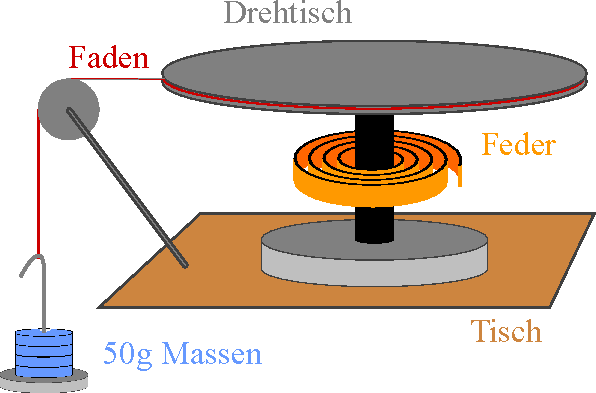
\includegraphics[width=0.4\textwidth, page=1,]{img/\versuchsnummer/Drehtisch.pdf}
    \caption{Versuchsskizze}
    \label{fig:drehtisch}
\end{figure}